\chapter{Introduction}
\label{Ch:intro}
This chapter introduces the project, first, by establishing the objective of the monograph and after that, giving a brief introduction to the concepts needed throughout the document. We divide these concepts into two parts: DESI project and Machine Learning. First, we introduce the project and the main aspects of the instrument and survey, such as the target selection and simulations. After that, we introduce machine learning concepts, particularly related to supervised learning and kernel methods.

\section{Objectives}
\subsection{General Objective}
\begin{itemize}
	\item Recover the true redshifts of Bright Galaxies using observational variables from the simulated DESI measurements as an input to kernel methods of machine learning, to improve the accuracy of DESI when used in the real world
\end{itemize}
\subsection{Specific Objectives}
\begin{itemize}
\item Characterize the dataset using a simple statistical and graphical procedure to select the set of meaningful features as input to the machine learning algorithms
\item Determine the set of computational parameters such as memory requirement, number of processors per node and size of dataset that performs the best on the cluster of the university restricted to constraints of resources, execution time and waiting time in the queue
\item Train and tune the hyper-parameter of the models by using grid-search and cross-validation
\item Test and select the best model based on performance on unseen data and model simplicity
\end{itemize}
\section{DESI Project}
The accelerated expansion of the universe is one of the most important phenomena in astrophysics, and in all modern physics, to such a point that it pushes forward the majority of the research done in observational cosmology \cite{Nord:2016plv}. DESI (Dark Energy Spectroscopic Instrument) will map one-third of the sky during a 5 years period\cite{Aghamousa:2016zmz}. DESI is a Stage IV ground-based dark energy experiment that will study baryon acoustic oscillations (BAO) and the growth of structure through redshift-space distortions (RSD) with a wide-area galaxy and quasar redshift survey. The survey will target four classes of extragalactic objects: Bright Galaxies (BGS), Luminous Red Galaxies (LRGs), Emission Line Galaxies (ELGs) and Quasi-stellar objects (QSOs) \cite{Aghamousa:2016zmz}. DESI is an instrument capable of taking up to 5000 simultaneous spectra in a range from 360 nm to 980 nm \cite{Aghamousa:2016sne}. 
LRGs will be observed up to a $z = 1.0$. To explore the universe in a higher redshift, DESI will target ELG of up to $z = 1.7$. Quasars will be observed as direct signals from the underlying dark the matter distribution, and, to higher redshifts, $2.1<z<3.5$, using the ly-$\alpha$ forest absorption. 

Before DESI stars to work, it needs simulations for its design, development, and testing. Some of this simulation focus on individual aspects, for example, hardware optimization, spectrographic analysis, fiber alignment, and target selection. In this project, we will use the result of the simulation of the redshifts of targets, and the simulation of the measurements of the instrument, to find the relationship between the expected measurement and actual measurement of the spectrograph.
\subsection{Targets}
The DESI survey will measure with high precision the baryon acoustic feature imprinted on the large-scale structure of the Universe, as well as the distortions of galaxy clustering due to redshift space effects. The survey will make spectroscopic observations of BGS, LRGs, ELG, and QSOs. To ensure highly efficient and spectroscopic completeness, the survey will select objects with spectral features expected to produce a reliable redshift determination or a Ly-$\alpha$ forest measurement within the DESI wavelength range \cite{Aghamousa:2016zmz}. Figure \ref{fig:targetsum} shows a summary of the properties of each DESI target class. 
\begin{table}[h!]
	\centering
	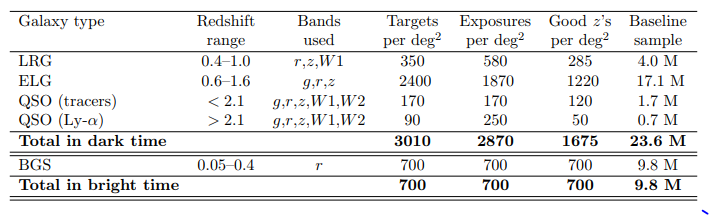
\includegraphics[width=1\linewidth]{TeX_files/Imagenes/target_sum}
	\caption{Summary of the properties of each DESI target class. The band listed are for the target selection, where $g$, $r$ and $z$ are optical photometry and $W1$ and $W2$ denote WISE infrared photometry \cite{Aghamousa:2016zmz}.}
	\label{fig:targetsum}    
\end{table}
\subsubsection{Bright Galaxy Sample}
The galaxy sample for the BGS will be a flux-limited, $r$-band selected sample of galaxies. The
magnitude limit is determined by the total amount of observing bright time and the exposure
times required to achieve our desired redshift efficiency. This target selection is, in essence, a
deeper version of the galaxy target selection for the SDSS main galaxy sample (MGS). We explore
the properties of the BGS target sample through mock catalogs created from numerical simulations.
These mocks have identical properties to the MGS at low redshift, including the luminosity function, color distribution, and clustering properties. \cite{Aghamousa:2016zmz}.
\subsubsection{Luminous Red Galaxies}
The lowest-redshift dark-time sample for DESI will come from targeting 350 candidate luminous
red galaxies (LRGs) per square degree. These objects are both high in luminosity and red in
rest-frame optical wavelengths due to their high stellar mass and lack of ongoing star formation.
They exhibit strong clustering and a relatively high large-scale-structure bias, which enhances the
amplitude of their power spectrum, and hence the BAO signal. Because of their
strong 4000 $\AA$  breaks and their well-behaved red spectral energy distributions, low-redshift LRGs
at $z < 0.6$ can be selected efficiently and their redshifts estimated based on SDSS-depth photometry. The BOSS survey has targeted 119 LRGs per $deg^2$ with $z \leq 0.6$ using SDSS imaging. DESI science analyses will incorporate existing BOSS spectroscopic samples (which cover 10,000
$deg^2$ of the DESI footprint) when available, as well as applying BOSS-like target selection algorithms
(in regions not yet covered) to target LRGs at low z \cite{Aghamousa:2016zmz}.
\subsubsection{Emission Line Galaxies}
Emission-line galaxies (ELGs) constitute the largest sample of objects that DESI will observe.
The galaxies exhibit strong nebular emission lines originating in the ionized (“H II”) regions
surrounding short-lived but luminous, massive stars. ELGs are typically late-type spiral and
irregular galaxies, although any galaxy actively forming new stars at a sufficiently high rate
will qualify as an ELG. Because of their vigorous ongoing star formation, the integrated
rest-frame colors of ELGs are dominated by massive stars, and hence will typically be bluer
than galaxies with evolved stellar populations such as LRGs. The optical colors of ELGs at
a given redshift will also span a larger range than LRGs due to the greater diversity of their
star formation histories and dust properties
\subsubsection{QSOs}
The highest-redshift coverage of DESI will come from quasars (a.k.a. quasi-stellar objects,
or QSOs), extremely luminous extragalactic sources associated with active galactic nuclei.
QSOs are fueled by gravitational accretion onto supermassive black holes at the centers of
these galaxies. The QSO emission can outshine that of the host galaxy by a large factor.
Even in the nearest QSOs, the emitting regions are too small to be resolved, so QSOs
will generally appear as point sources in images. These are the brightest population of
astrophysical targets with a useful target density at redshifts $z > 1$ where the population
peaks.
\subsection{Simulations}
Simulations are needed throughout the design, development, and operations of DESI. Some of
these focus on individual aspects, e.g., to optimize a particular piece of the hardware design or
to tune an individual algorithm. Other simulations provide mock data for the spectral extraction
pipeline development prior to obtaining real data. End-to-end simulations will ensure system-level
integration and scaling of the software, while also validating the design performance as a whole.
Cosmological simulations are needed as input for particular pieces that require realistic cosmology
to test their performance \cite{Aghamousa:2016sne}.
\subsubsection{Cosmological Simulations}
Cosmological simulations are critical inputs for the development, testing, and validation of the full
DESI pipeline. In particular, they are essential to
\begin{itemize}
	\item understand the effect of the tiling and fiber assignment strategies
	\item model the radial selection function of the different targets for the development of the large-scale structure catalog.
	\item  provide a realistically clustered mock input catalog for algorithm development
	\item serve as input for the end-to-end simulation pipeline for system level testing
\end{itemize}
The cosmological simulations as needed by DESI are constructed with a multi-step procedure.
First, given a cosmological model, an N-body simulation is run using either baryons plus dark matter
or solely dark matter. Second, galaxies and quasars are populated within this N-body simulation:
Gas-hydrodynamical simulations need a way of identifying the objects, while solely dark matter
simulations require a scheme such as a statistical halo occupation distribution (HOD) model or
a physical semi-analytic galaxy formation model \cite{Aghamousa:2016sne}.
\subsubsection{Instrument Simulations}
Instrument simulations guide the hardware design process and provide inputs for the spectral
pipeline development. This is optimized both at the high-level to ensure that DESI meets the science
requirements, and at the low-level for where the spectral extraction pipeline places requirements
on the hardware design \cite{Aghamousa:2016sne}. 
\begin{figure}[h!]
	\centering
	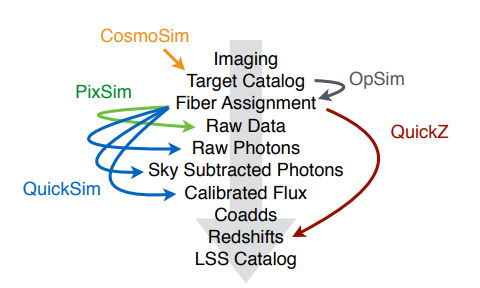
\includegraphics[width=1\linewidth]{TeX_files/Imagenes/desi_sim}
	\caption{Diagram of different types of simulations for testing and improving DESI \cite{Aghamousa:2016sne}}
	\label{fig:desisim}
\end{figure}
Figure \ref{fig:desisim} shows a diagram of the different simulation used to test and optimize DESI. This simulations are:
\begin{itemize}
	\item CosmoSIM: input cosmology simulations to produce mock target catalogs.
	\item PixSim: pixel-level simulations of raw data to be used for spectroscopic pipeline development and study of detailed systematics.
	\item QuickSim: a fast spectral simulator that emulates the DESI spectroscopic resolution and throughput. It propagates signal, sky, and detector noise but bypasses the computationally expensive raw data pixel simulations and extractions.
	\item OpSim: a survey simulator that traces what tiles would be observed in what order based upon the real next field selector and a Monte Carlo realization of weather and observing conditions.
	\item QuickZ: an ultra-fast simulator that applies DESI efficiencies to an input target catalog to generate an output redshift catalog.
\end{itemize}
\section{Machine Learning}
Machine learning plays a key role in many areas of science, finance, and industry, some examples may be the prediction of medical conditions and diseases, prediction of price of a stock on the basis of company performance and economic data or estimating the amount of glucose in the blood of a diabetic person from the infrared absorption spectrum of the blood.

In general, the problem of machine learning consist typically of having a set of measurements, that can be either quantitative (the measurement of an instrument or a stock price) or categorical (such as a class, or category) that we want to predict based on a set of \textbf{features}, for example, the performance metrics of a company. For doing this, we have a \textbf{training} set of data, in which we know the relation between the outcome and the features, from this, we build a prediction model, or \textbf{learner}, and then use the model to predict the outcomes of features in a \textbf{test} set, to see if the model is able to \textbf{generalize} what it \textit{learned} from the training set. A good learner is one that accurately predicts such an outcome \cite{Hastie2009}. This particular way of learning is called learning from example, or \textit{\textbf{supervised learning}}. There are other forms of learning, such as unsupervised learning and reinforcement learning, this two forms of learning will not be discussed in this monograph.

More formally, we can describe the general model of learning from example through three components\cite{Vapnik2000}:
\begin{enumerate}[I]
	\item A generator ($G$) of random vectors $x \in R^n$, drawn independently from a fixed but unknown probability distribution function F(x)
	\item A supervisor ($S$) who returns an output value $y$ to every input vector $x$ according to a conditional distribution function $F(y|x)$, also fixed but unknown. This is the general case, which includes the case where the supervisor uses a function $y = f(x)$.
	\item A learning machine ($LM$) capable of implementing a set of functions $f(x, \alpha), \alpha \in \Lambda$, where $\Lambda$ is a set of parameters.
\end{enumerate}
\begin{figure}[ht!]
	\centering
	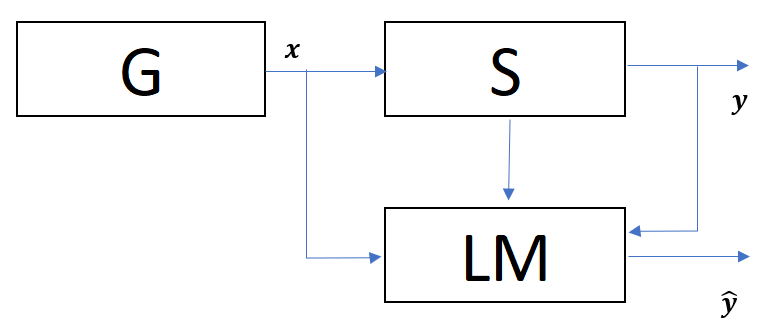
\includegraphics[width=0.7\linewidth]{TeX_files/Imagenes/ML_diagram}
	\caption{A model of learning from examples \cite{Vapnik2000}.}
	\label{fig:mldiagram}
\end{figure}
The description of the process is shown in figure \ref{fig:mldiagram}. In order to choose the best available approximation to the supervisor´s response, one measures the \textit{loss} or discrepancy between the response provided by the $LM, \, \, f(x, \alpha)$ and the supervisor's response ($y$), $L(y, f(x, \alpha))$. Consider the expected value of the loss, give by the \textit{Risk Functional}:
\begin{equation}
R(\alpha) = \int L(y, f(x, \alpha))dF(x, y).
\end{equation}
The goal is to find the function $f(x, \alpha_0)$ that minimizes the risk functional $R(\alpha)$, in the situation where the joint probability distribution function $F(x, y)$ is unknown and the only available information is contained in the \textbf{training set} \cite{Vapnik2000}. The problem of supervised learning can be divided in three classes: the problem of patter recognition, regression estimation, and density estimation. 
\subsubsection*{Patter recognition}
In this problem the supervisor's response is categorical of two values $y = {0, 1}$. For example, in a classification problem, whether a picture contains a dog or not. The loss function in this case is 
\begin{equation}
L(y, f(x,\alpha)) = \begin{cases} 0, & \mbox{if } y= f(x, \alpha) \\ 1, & \mbox{if } y \ne f(x, \alpha) \end{cases}
\end{equation}
\subsubsection*{Regression Estimation}
Let the supervisor´s answer $y$ be a real value, and let $f(x, \alpha), \alpha \in \Lambda$ be a set of real functions that contains the \textbf{regression function} 
\begin{equation}
f(x, \alpha) = \int y dF(y|x).
\end{equation}
The loss function for this problem is
\begin{equation}
L(y, f(x,\alpha)) = (y - f(x, \alpha))^2 .
\end{equation}
\subsubsection*{Density Estimation}
Finally, consider the problem of density estimation from a set of densities $p(x, \alpha), \alpha \in \Lambda$. For this problem we consider the following loss function
\begin{equation}
L(p(x, \alpha)) = -\log p(x, \alpha).
\end{equation}

In this monograph, we will make use of the regression problem, since we want to find the correct redshift from a series of observational features. For requirements of the project, the algorithms used have to be simple and keep the number of parameters low. The main algorithms for regression in machine learning include kernel method and artificial neural networks (NN). In recent years NNs have been used to solve lots of machine learning problems, however, they require an incredibly large number of parameters (as in deep learning where the number of parameters can reach the millions). Therefore, the kernel methods will be explored while the NNs will be left out. 
\subsection{Kernel Methods}
The theory and algorithms of machine learning are very well developed for the case of linear models. However, real-world data often requires nonlinear methods to detect the kind of patterns and dependencies that allow successful predictions. This is where the kernel is used, by using a positive definite kernel, we can have the best of both worlds. The kernel corresponds to a dot product in a feature space, in this space, the estimation method is linear\cite{Hofmann2008}. 

Suppose we are given empirical data
\begin{equation}
(x_1, y_1), ..., (x_n, y_n) \in \mathcal{X} \times \mathcal{Y}.
\end{equation}
Here, the domain $\mathcal{X}$ is the set of \textit{inputs}, where the predictor variables, $x_i$, are taken from; the $y_i \in \mathcal{Y}$ are called targets. Apart from being a set, $\mathcal{X}$, most have a structure that allows us to measure the similarity between input points so that the method can \textit{generalize} to unseen data points. In the case of binary classification, for example, given a new input $x\in \mathcal{X}$, we want to predict the corresponding $y \in {\pm 1}$. Generalization means we want to predict a $y$ such as the pair $(x, y)$ is in some sense \textit{similar} to the training examples. To this, we need similarity measures in $\mathcal{X}$ and ${\pm 1}$. The letter is easier since in the target space two values can only be identical or different. For the input space, we need a 'similarity' function 
\begin{equation}
k: \mathcal{X}\times\mathcal{X} \rightarrow \mathbb{R}, \,\,\,\,\,\,\,\, (x, x') \rightarrow k(x, x')
\end{equation}
satisfying, for all $x, x' \in \mathcal{X}$,
\begin{equation}
k(x, x') = \langle \Phi (x), \Phi(x')\rangle ,
\end{equation}
where $\Phi$ maps into some dot product space $\mathcal{H}$, sometimes called the \textit{feature space}. The similarity measure $k$ is called a \textit{kernel}, and $\Phi$ is called its \textit{feature map} \cite{Hofmann2008}. The advantage of using such a kernel as a similarity measure is that it allows us to construct algorithms in dot product spaces. The \textit{kernel function} can be in practical uses one of the following:

\begin{align}
\text{linear} &= \langle x, x' \rangle. \\
\text{polynomial} &= (\gamma \langle x, x' \rangle + r )^d .\\
\text{rbf} &= \exp(-\gamma  ||x - x'||^2 ) .\\
\text{sigmoid} &= \tanh(\gamma \langle x, x' \rangle + r ) .\\
\end{align}

Where $\gamma, d,$ and $r$ are hyper-parameters that must be tuned by hand and $\langle x, x' \rangle$ represents a dot product in the corresponding space. 
\subsection{Support Vector Machines used for Regression}
A support vector machine constructs a hyperplane or set of hyperplanes in a high or infinite dimensional space, which can be used for classification, regression or other tasks. Intuitively, a good separation is achieved by the hyperplane that has the largest distance to the nearest training data points of any class (so-called functional margin), since in general the larger the margin the lower the generalization error of the classifier \cite{SMOLA2004}. For the case of a regressor, the basic idea is the following: in $\epsilon-SV$ regression \cite{Vapnik2000}, our goal is to find a function $f(x)$ that has at most $\epsilon$ deviation from the actually obtained targets $y_i$ for all training data, and at the same time is as flat as possible. In other words, we do not care about errors as long as they are less than $\epsilon$, but will not accept any deviation larger than this. For the simpler case, we begin by describing the case of a linear function as an example, taking the form
\begin{equation}
f(x) = \langle w, x \rangle + b.
\end{equation}
In this case, \textit{flatness} means that one seeks for small $w$. One way to ensure this is to write the optimization problem as follows:
\begin{align}
\text{minimize} \,\,\, \, &\frac{1}{2}||w||^2 \\
\text{subject to} \,\,\,\, &
\begin{cases}
y_i - \langle w, x \rangle  - b & \leq \epsilon \\
\langle w, x \rangle  + b - y_i &\leq \epsilon
\end{cases}
\end{align}
This assumes however, that such a function $f$ exists, but it may not be the case where all the data points can be fit into a tube of size $2\epsilon$, therefore, one can introduce slack variables $\zeta$ and $\zeta^*$ to cope with the otherwise infeasible constraints of the previous optimization problem. Hence we arrive at the following formulation:
\begin{align}
\text{minimize} \,\,\, \, &\frac{1}{2}||w||^2 + C\sum_{i = 1}^{l} (\zeta_i + \zeta^{*}_{i}) \\
\text{subject to} \,\,\,\, &
\begin{cases}
y_i - \langle w, x \rangle  - b & \leq \epsilon + \zeta_i \\
\langle w, x \rangle  + b - y_i &\leq \epsilon + \zeta^{*}_i \\
\zeta_i, \zeta^{*}_{i} &\geq 0
\end{cases}
\end{align}
The constant $C$ determines the trade-off between the flatness of $f$ and the amount up to which deviations larger than $\epsilon$ are tolerated. 
\begin{figure}[th!]
	\centering
	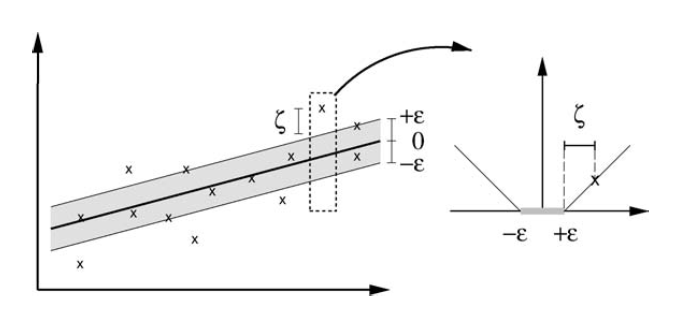
\includegraphics[width=1\linewidth]{TeX_files/Imagenes/svr_graph}
	\caption{The soft margin loss setting for a linear SVM \cite{Hofmann2008}}
	\label{fig:svrgraph}
\end{figure}
Figure \ref{fig:svrgraph} shows the schematics of a linear SVM used for regression, the grey zone represents were the loss function does not account any penalty and the $\zeta$ shows the tolerance to deviations. 

For non-linear functions, the data can be mapped into a high dimensional space, called kernel space. Therefore, replacing all instances of $x$ in the previous equations with $k(x_i, x_j)$ yields the formulation of the optimization problem. This is a complete subject of mathematics and we can not dig further, but generally speaking, the optimization problem is solved using Lagrange multipliers and the Karush-Kuhn-Tucker conditions. The objective of the procedure is to find the weights $w$. The use of this mathematical tools results in that the $w$ can be written explicitly as a linear combination of the so-called \textbf{support vectors}, which are training samples that lie outside the boundary of the tube. In a sense, the complexity of a function's representation by SVs is independent of the dimensionality of the input space and depends only on the number of support vectors\cite{Hofmann2008}. The decision boundary function is:
\begin{equation}
\sum_{i = 1}^{n} (\alpha_i - \alpha_{i}^{*})k(x_i, x) + b,
\end{equation}
These parameters correspond to the dual coefficients of the optimization problem (also called Lagrange multipliers), $\alpha, \alpha_{i}^{*}$, the support vectors $x_i$ and the independent term, the intercept $b$. Note that this is a hyper-plane on the feature space. Therefore, the solution in classification or regression is contained in this set of parameters only. 
\subsection{Kernel Ridge Regression}
Kernel ridge regression combines Ridge Regression with the kernel trick. It thus learns a linear function in the space induced by the respective kernel and the data. For non-linear kernels, this corresponds to a non-linear function in the original space \cite{krr}. The form of the model learned by this method is identical to support vector regression but with different loss functions. In ridge regression, the regression coefficients are shrunk by imposing a penalty on their size. The ridge coefficients minimize a penalized residual sum of squares:
\begin{equation}
w = \arg \min_{w} \left[ \sum_{i = 1}^{N}(y_i - b - \langle w, x\rangle) + \lambda \sum_{j = 1}^{p} w_{i}^{2}\right].
\end{equation}
Here $\lambda \geq 0$ is a complexity parameter that controls the amount of shrinkage: the larger the value of $\lambda$, the grater the amount of shrinkage. As the $\epsilon$-insensitive loss functions of SVRs, the ridge solutions are not equivariant under scaling of the inputs, and so one normally standardizes the inputs before solving. 

These methods will be used to correct the redshift prediction of the DESI instrument. To do this, it is therefore necessary to properly select the features, scale the data and tune the hyper-parameters of the algorithms. We will explain how to do this in the following chapter. 